% LuaLaTeX
\pdfvariable minorversion=7
\documentclass[10pt]{article}

% Packages
\usepackage[no-math]{fontspec}
\usepackage{geometry}
\usepackage{hyperref}
\usepackage[backend=biber]{biblatex} % we use the biber implementation of biblatex for bibliographies
%\usepackage[nonumberlist, toc]{glossaries}
\usepackage{graphicx}
\usepackage{pdfpages}
\usepackage{booktabs}
\usepackage{float}
\usepackage{subcaption}
\usepackage{fancyhdr}
\usepackage{amsmath}
\usepackage{siunitx}
\usepackage{multirow}

% Formatting
\geometry{letterpaper, portrait, margin=.85in}
\defaultfontfeatures{Ligatures=TeX}
\setmainfont[
    BoldFont       = Avenir Medium,
    ItalicFont     = Avenir Book Oblique,
    BoldItalicFont = Avenir Medium Oblique
]{Avenir Book}
\setmonofont{Andale Mono}
\sisetup{detect-all} % used by siunitx to always typeset units in the font of the current environment
\urlstyle{same}

\newcommand\theteamname{Midnight Sun Solar Car Team} % should not change normally
\newcommand\theuniversityname{University of Waterloo} % should also not change normally
\newcommand\theteamwebsite{www.uwmidsun.com} % should also not normally change
\newcommand\theteamphone{(519) 888-4567 x32978} % should also not normally change

\newcommand\thetitle{Battery Protection Tech Report} % <--------------- add the title
\newcommand\thesubtitle{Electrical} % <--------------- add a subtitle or leave the field empty
\newcommand\theauthor{Minghao Ji} % <--------------- add an author with contact info or comment this line
\newcommand\theauthorcontact{minghao.ji@uwmidsun.com} % <--------------- add author's email or leave the field empty
\newcommand\thedate{\today} % <--------------- update the date, use this format

\pagestyle{fancy}
\renewcommand{\headrulewidth}{0pt}
\lhead{\thetitle}
\rhead{\theteamname}

\begin{document}

% Title Page
\begin{titlepage}
\large
\vspace*{2cm}
\centering

\includegraphics[width=.25\textwidth]{./figures/midnightSunLogoCircle.png} \\
\vspace{1.5cm}
{\LARGE \theteamname} \\
\theuniversityname \\
\vspace{2.2cm}
{\LARGE MSXII} \\
\vspace{0.4cm}
{\huge\bfseries \thetitle} \\
\vspace{0.2cm}
{\LARGE \thesubtitle} \\
\vspace{2.2cm}
\ifdefined \theauthor
\par Prepared by: \\
\theauthor \\
\theauthorcontact \\
\fi
\thedate \\
\vfill
\theteamwebsite \\
\theteamphone
\end{titlepage}

% Main Matter
\tableofcontents
\newpage
%\listoffigures % <-------------- uncomment for list of figures
%\listoftables % <-------------- uncomment for list of tables

\section{Overview}

\subsection{5.2.E.1: Battery Approval Form}

See attached form

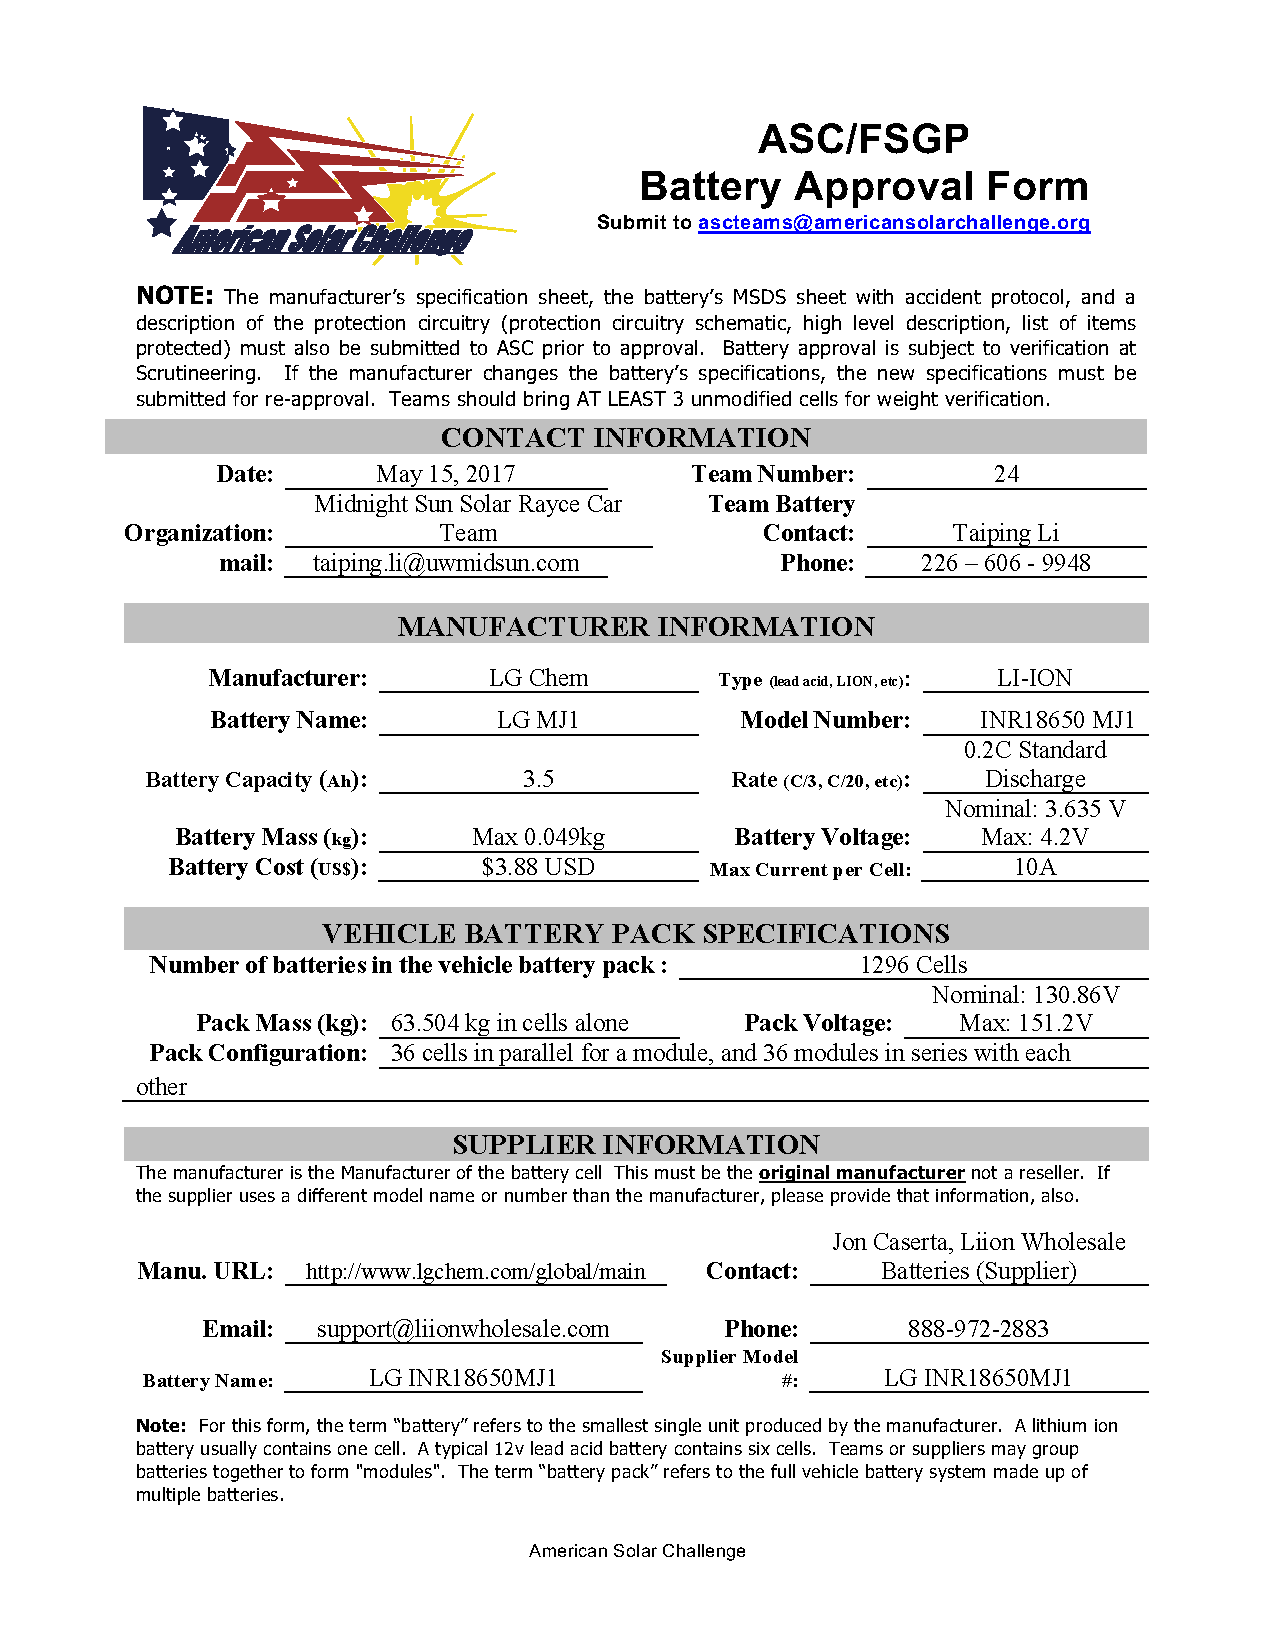
\includepdf[pages={-}]{forms/battery_approval_form.pdf}

\subsection{5.2.E.2: Battery Pack Configuration}

\begin{table}[!htbp]
\begin{tabular}{|l|l|}
\hline
\textbf{Cells per module}    & 36   \\ \hline
\textbf{Modules per string}  & 36   \\ \hline
\textbf{Strings in parallel} & 1    \\ \hline
\textbf{Total cell count}    & 1296 \\ \hline
\end{tabular}
\end{table}

\subsection{5.2.E.3: Over temperature set points}

\begin{table}[!htbp]
\begin{tabular}{|l|l|}
\hline
\textbf{Over temperature set point (charge) ($^{\circ}$C)}    & 45 \\ \hline
\textbf{Over temperature set point (discharge) ($^{\circ}$C)} & 60 \\ \hline
\end{tabular}
\end{table}

\subsection{5.2.E.4: Under voltage set points}

\begin{table}[!htbp]
\begin{tabular}{|l|l|}
\hline
\textbf{Under voltage set point (V)}    & 2.5 \\ \hline
\end{tabular}
\end{table}

\subsection{5.2.E.5: Over voltage set points}

\begin{table}[!htbp]
\begin{tabular}{|l|l|}
\hline
\textbf{Over voltage set point (V)}    & 4.2 \\ \hline
\end{tabular}
\end{table}

\subsection{5.2.E.6: Over current set points}

\begin{table}[!htbp]
\begin{tabular}{|l|l|}
\hline
\textbf{Over current set point (A)}    & 110 \\ \hline
\end{tabular}
\end{table}

\subsection{5.2.E.7: BPS Block Diagram}

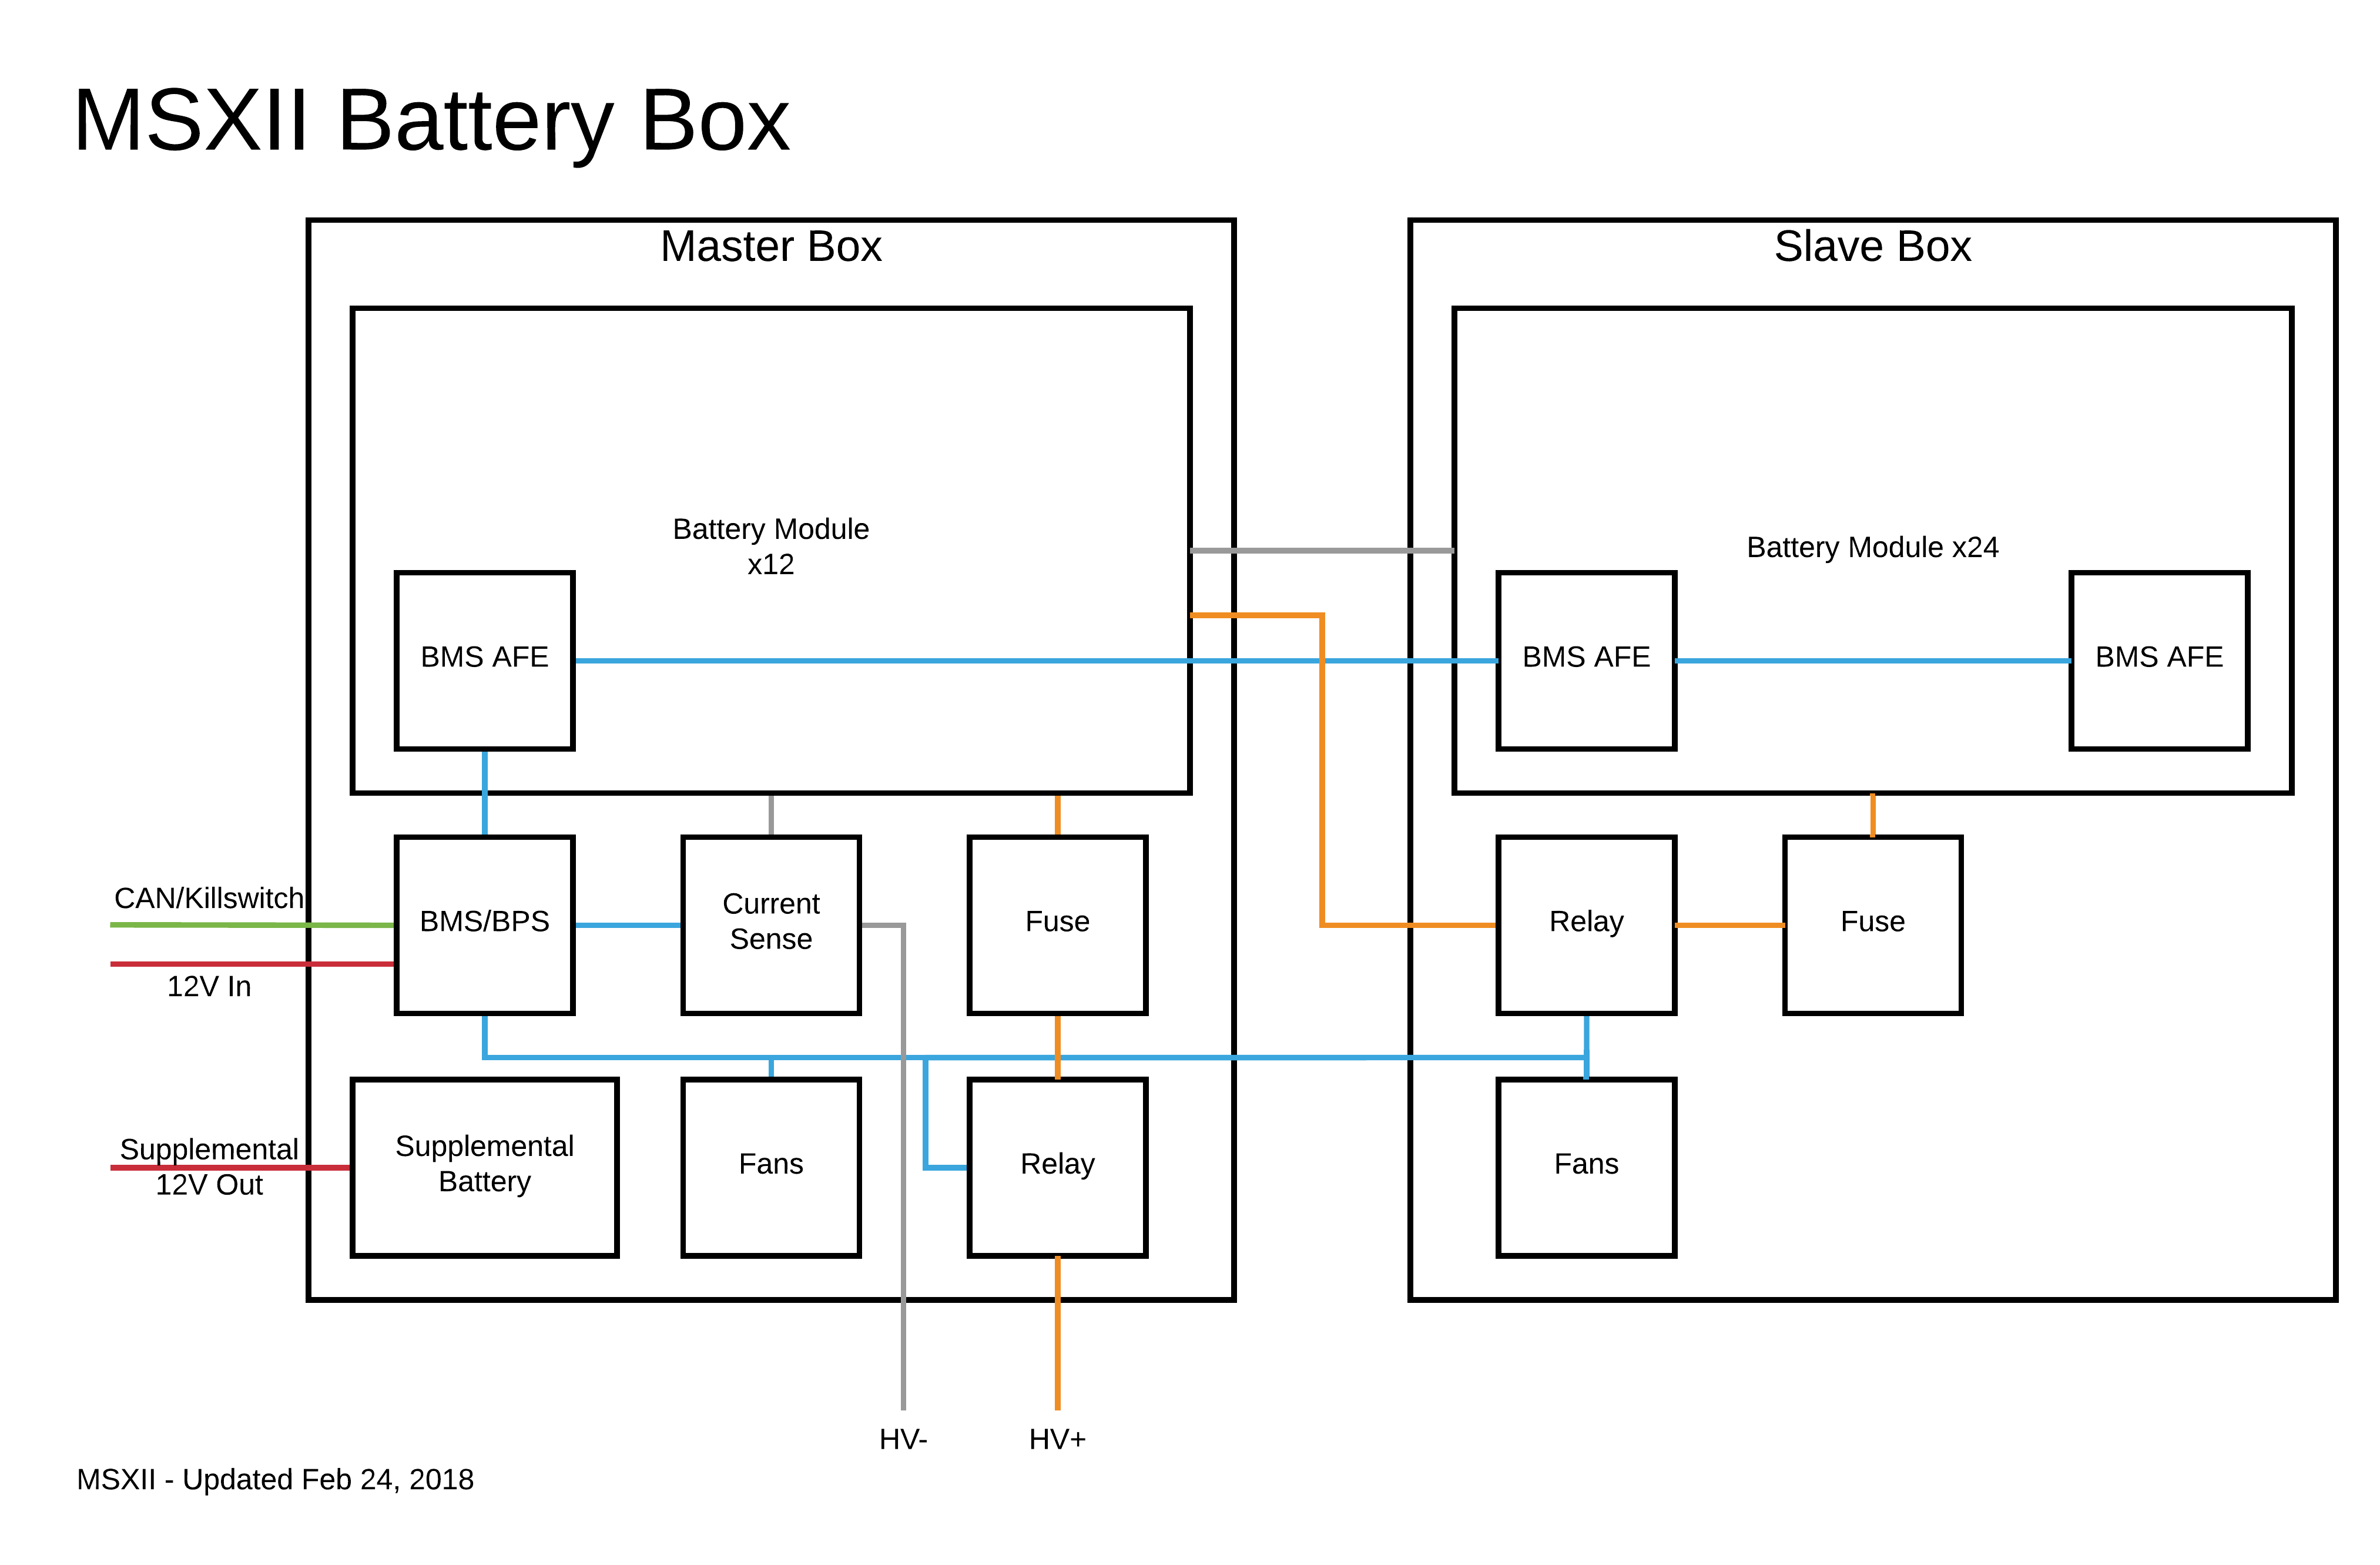
\includegraphics[width=1\textwidth]{./figures/msxii-electrical-battery-box-block-diagram.png}

\subsection{5.2.E.8: BPS Operation}

The BPS will monitor for each of the fault conditions on each iteration of its
\texttt{main} loop. We use the \texttt{LTC6804-1} in a daisy-chain
configuration to read the voltages and temperatures of each battery module, and
we use an ADC and a shunt resistor to measure the current.

If it detects a fault condition, it will raise a BPS fault error, which is
broadcast on the CAN bus. This message is processed by our
\texttt{power distribution} and \texttt{driver controls} boards. It will also
drive the two pack fans.

The only way to clear a fault will be to power off the car, which will result
in the car undergoing the proper power-sequencing steps.

\subsection{5.2.E.9: Rendering Firmware Static}

We will seal the programming header of the BPS microcontroller, which will
make it impossible to reprogram the firmware.

\subsection{5.2.E.10: Driver dash and BPS fault indicator}

\subsubsection{Driver Dash}

When the \texttt{Lights} board receives the BPS fault message, it turns on the
Strobe light mounted on the roof of the car.

There is an LED on the driver dash. When the \texttt{Driver Controls} board
receives the BPS fault message, it turns on this LED.

\subsubsection{External Cutoff switch}

The External Cutoff switch is monitored by the BPS. Pressing the External
Cutoff switch results in the HV rails being disconnected, and disconnects the
unprotected rail.

When the BPS detects that the switch is pressed, it raises a BPS fault, and
the normal fault behaviour occurs.

% Bibliography
%\pagebreak
%\printbibliography

% Appendix
\pagebreak
\appendix

\end{document}
